%% eval.tex
%% $Id: eval.tex 5 2005-10-10 20:55:48Z bless $

%%%%%%%%%%%%%
\chapter{Ergebnisbeschreibung}
\label{ch:evaluation}
%%%%%%%%%%%%%

Nach der Durchführung der Studie gilt es, die Ergebnisse dieser auszuwerten und einzuordnen. Hierfür werden mehrere erhobenen Daten betrachtet. Die Evaluation der Studienergebnisse besteht zunächst aus der Beschreibung der Charakteristika der Probandengruppe. Anschließend werden die Ergebnisse der Erhebungen beschrieben. Eingegangen wird hierbei auf die Ergebnisse der Fragebögen, sowie der Abschließenden Fragerunde. Abschließend werden die Ergebnisse der Fragebögen mit den Einschätzungen der Fragerunde in Verbindung gebracht. 


\section{Deskriptive Statistik}
Es nahmen acht Probanden an der Vergleichsstudie teil. Diese befinden sich zum Zeitpunkt der Durchführung im Alter von 23 bis 37 Jahren. Das durchschnittliche Alter beträgt 29. Die Probandengruppe setzt sich aus fünf Frauen und 3 Männern zusammen. Die Probanden sind wissenschaftliche Mitarbeiter, Promotionsstudenten oder Doktoren aus dem medizinischen Bereich. 

Folgende Aussagen lassen sich über die Gewohnheiten und Technologienutzung der Probanden ableiten. Die Mehrheit verwendet ein- oder mehrmals am Tag Chat-Technologien. Ein Proband nutzt Chat-Technologien 
einmal im Monat oder seltener. Die verwendeten Chat-Technologien setzen sich aus Whatsapp, Telegram, Facebook Messenger, Instagram, Threema, Apple Nachrichten, Line und Slack zusammen. Die meistgenutzten Chat-Technologien innerhalb der Probandengruppe sind Whatsapp und Facebook Messenger. Verwendet werden diese Anwendungen hauptsächlich auf dem Smartphone oder Laptop bzw. Desktop Computer. 

Die Nutzung von Chatbots ist innerhalb der Probandengruppe wenig verbreitet. Diese werden von zwei Probanden einige Male pro Woche und einmal im Monat oder weniger genutzt. Genutzt werden der Nachrichtenbot der Tagesschau und ein Chatbotdienst für den Kundenservice der Firma ASOS. Bedient werden diese Chatbotdienste auf dem Smartphone sowie Laptop bzw. Desktop Computer. 

Innerhalb der Probandengruppe wurde Experience Sampling bereits mehrheitlich genutzt. Drei Probanden gaben an noch nie oder nur gelegentlich Experience Sampling verwendet zu haben. Fünf Probanden haben bereits Experience Sampling öfters bis regelmäßig genutzt. Für Experience Sampling kamen die Anwendungen MovisensXS, Menthal und Whatsanalyzer zum Einsatz. Genutzt wurden diese auf dem Smartphone oder Laptop bzw. Desktop Computer. 

Hinsichtlich der Vorerfahrungen bezüglich MovisensXS lassen sich für die Probandengruppe folgende Aussagen treffen. Wie in Grafik \ref{movisensXSErfahrung} zu sehen ist, besitzt ein Proband keinerlei Erfahrungen mit MovisensXS. Die restlichen Probanden nutzen das Programm gelegentlich bis regelmäßig. Die Nutzung von MovisensXS beschränkt sich auf das Zuordnen von Probanden, Teilnahme an Studien, sowie kleinen Anpassungen einer bereits bestehenden Studie. 

\begin{figure}[h]
\centering
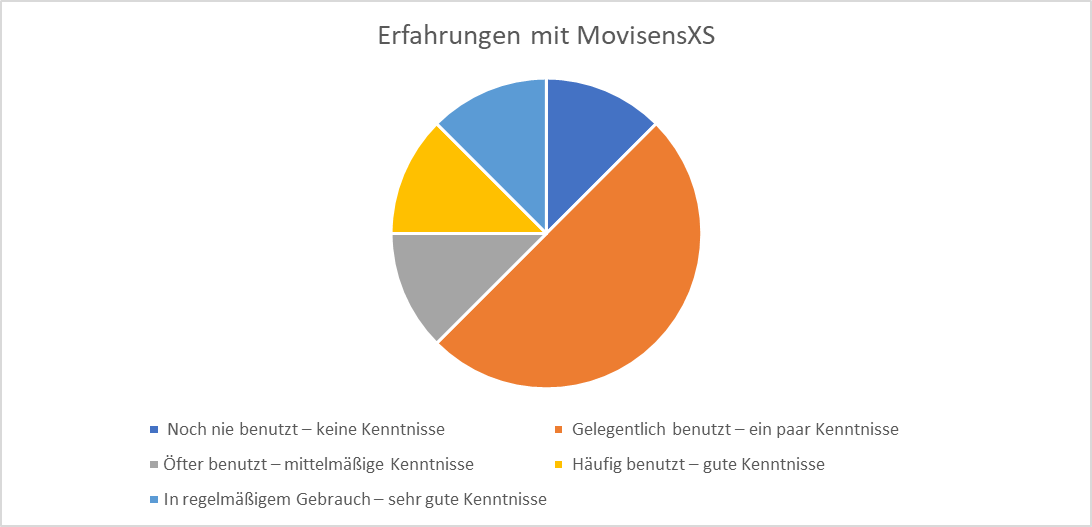
\includegraphics[width=1\textwidth]{pictures/diagramme/movi}
\caption{Angaben der Probanden bezüglich ihrer Erfahrungen mit dem Programm \emph{MovisensXS}}
\label{movisensXSErfahrung}
\end{figure}

Basierend auf dieser Probandengruppe ist es für die Überprüfung der aufgestellten Hypothesen bedeutend, die jeweiligen Probanden zu framen. Hierfür werden zunächst Sinn der Studie und diverse Begriffe erläutert. Anschließend machen sich die Probanden zunächst mit dem jeweiligen Programm vertraut, welches betrachtet werden soll. Hierfür wird eine Aufgabe gestellt, die durch das Programm führt und den Probanden beim explorieren des jeweiligen Programms und dessen Funktionen anleitet. Während der Nutzung und der Bearbeitung der gestellten Aufgaben, werden Emotionen und Motivationen durch Kommentare des Probanden erfasst. Abschließend wird nach der aufgabengesteuerten Nutzung eines Programms eine erste Einschätzung in Form eines Fragebogens erfasst. Nach Bearbeitung aller Aufgaben und Verwendung beider Programme, werden die Programme in einer abschließenden Fragerunde miteinander verglichen. Dabei wird auf wesentliche Unterschiede beider Programme eingegangen. Erfasst werden hierbei die Einschätzung der Probanden, welche Eigenschaften sie im Vergleich als besonders Hilfreich, nicht Hilfreich empfanden. Auch welche Eigenschaften ihnen gefallen oder welche sie vermisst haben. Diese Einschätzungen werden in Relation zu den Ergebnissen der Fragebögen gesetzt um diese zu verargumentieren.

%%%%%%%%%%%%%%%%%%%%%%%%%%%%%%%%%%%%%%%%%%%%%%%%%%%%%%%%%%%%%%%%%%%%%%%%%%%%%%%%%%%%%%%%%%%%%%%%%%%%%%
%%%%%%%%%%%%%%%%%%%%%%%%%%%%%%%%%%%%%%%%%%%%%%%%%%%%%%%%%%%%%%%%%%%%%%%%%%%%%%%%%%%%%%%%%%%%%%%%%%%%%%

\section{Beschreibung der Ergebnisse der Zwischenfragebögen}

Zunächst werden die Ergebnisse der Fragebögen betrachtet. Diese werden in verschiedene Kategorien eingeordnet, in denen sich die Ansätze maßgeblich unterscheiden. Die Einschätzungen der abschließenden Fragerunde der Studie werden ebenfalls betrachtet. Abschließend werden die Ergebnisse verknüpft und im Kontext der aufgestellten Hypothesen diskutiert. 

%%%%%%%%%%%%%%%%%%%%%%%%%%%%%%%%%%%%%%%%%%%%%%%%%%%%%%%%%%%%%%%%%%%%%%%%%%%%%%%%%%%%%%%%%%%%%%%%%%%%%%

\subsection{Konstruktionsprinzip und Konfigurationsprinzip}

Die Prototypen \emph{TherapyBuilder} und \emph{MovisensXS}, der Studie, unterscheiden sich maßgeblich in der Herangehensweise der Einstellung der Trigger. Während \emph{TherapyBuilder} das Konfigurationsprinzip verfolgt, nutzt \emph{MovisensXS} das Konstruktuionsprinzip. Die Studienergebnisse beider Ansätze werden zunächst getrennt betrachtet. Für diese Betrachtung werden vorerst die Ergebnisse der Fragebögen herangezogen. Abschließend erfolgt die Gegenüberstellung beider Ansätze. 

\subsubsection{Ergebnisbeschreibung des Konstruktionsprinzips}

Das Konstruktionsprinzip bietet das Einstellen der Trigger durch das Zusammensetzen und Verschalten einzelner Blöcke mit unterschiedlichen Funktionen. Wie in Abbildung \ref{konstruktion} dargestellt, bildet sich aus der Anordnung ein Baum aus verschiedenen Blöcken. Die Blöcke unterscheiden sich farblich und folgen dem Ampelprinzip.  

\begin{figure}[h]
\centering
\includegraphics[width=1\textwidth]{pictures/konstruktion}
\caption{Das Konstruktionsprinzip des MovisensXS. Blöcke werden miteinander verschaltet.}
\label{konstruktion}
\end{figure}

Die Probanden gaben nach der Aufgabenbearbeitung an, dass sie die Darstellung der Trigger als zumeist verständlich empfanden mit einer leichten Tendenz zu zum Teil verständlich. Dies wird auch durch die Freitext-Aussagen der Probanden gestützt. Fünfundsiebzig Prozent der Probanden gingen auf die positive Auswirkung der farblichen Kodierung ein. Zum einen wurde beschrieben, dass diese die Orientierung innerhalb des Baumes erleichtern und die Funktion sowie Abfolge der Bausteine gut beschreiben.

Die Verständlichkeit der Einstellungsmöglichkeiten der Trigger wurde von den Probanden sehr unterschiedlich bewertet. Im Schnitt wird diese als zum Teil verständlich und zumeist verständlich empfunden. Positiv wurde von einem Probanden die vielen möglichen Trigger-Optionen hervorgehoben.

Während des Durcharbeitens der Aufgaben wurden die Probanden in der Trigger-Ansicht mit Verzweigungen zwischen einzelner Konversationen konfrontiert. Diese wurden im MovisensXS als zum Teil verständlich empfunden. Diese Auswertung findet sich auch in den Aussagen wieder. Die Hälfte der Probanden gibt an, dass die Baumdarstellung bei vielen Bausteinen schnell unübersichtlich wirkt. 

Innerhalb des Baumes kann abgeleitet werden, welche Konversationen im Laufe des Therapiemoduls gestartet werden. Das Auffinden dieser Konversationen bewerteten die Probanden als eher gut. Dies findet sich auch in der bereits erwähnten Aussage der Probanden über die Unübersichtlichkeit der Darstellung wieder. 

Auch empfanden es die Probanden als eher schwierig die zeitliche Abfolge der Konversationen nachzuvollziehen. Im Schnitt bewerteten sie auch diese eher gut mit leichter Tendenz zu mäßig. Ein Proband beschrieb, dass der Baum nicht auf den ersten Blick erkennen lässt, was dieser Bedeutet. Ein weiterer merkte an, dass die Darstellung für den entsprechenden Zweck nicht sehr intuitiv ist. 

Das Anordnen der Bausteine zur Konfiguration der Trigger empfanden die Probanden im Schnitt gut verständlich. Dies wurde auch von den Probanden positiv hervorgehoben. Zwei Probanden beschreiben, dass das Baukasten-Prinzip die Konfiguration erleichtert. Ein Proband weißt ebenfalls auf die bereits erwähnte Vielfalt der Trigger-Optionen hin. Darüber hinaus wurde von knapp achtunddreißig Prozent die Anordnung der Bausteine via Drag and Drop positiv hervorgehoben.

Die Abhängigkeiten ließen sich hingegen nicht so gut erkennen. Im Schnitt tendiert die Einschätzung der Probanden eher zu einer eher guten Darstellung der Abhängigkeiten zwischen verschiedenen Konversationen. Dies kann erneut mit der, von den Probanden mehrfach genannten, Unübersichtlichkeit in Verbindung gebracht werden. 

Insgesamt empfanden die Probanden die Übersichtlichkeit der Therapie und deren Verlauf als eher mäßig. Ein Proband gab an, dass die Therapie für ihn schlecht zu überschauen ist. Die restlichen Probanden hingegen bewerteten diese zwischen sehr gut bis eher gut. Dies spiegelt sich wiederum in der Aussage über die fehlende Übersichtlichkeit innerhalb der Baum-Darstellung wieder. Dies wurde - wie bereits erwähnt - von fünfzig Prozent der Probanden angemerkt. 


\subsubsection{Ergebnisbeschreibung des Konfigurationsprinzip}

Im Vergleich zum oben beschriebenen Konstruktionsprinzip, verwendet das Konfigurationsprinzip hauptsächlich eine Oberfläche in der Einstellungen via Steuerelemente vorgenommen werden. Diese werden durch Formulare bereitgestellt wie in Abbildung \ref{konfiguration} verdeutlicht. Verschachteln von Triggern geschieht durch das Hinzufügen eines neuen Triggers zur jeweiligen Konversation. Basierend auf diesen Einstellungen wird ein Element im Zeitstrahl erzeugt, welches darstellt, wann eine Konversation gestartet wird, die Anzahl der Wiederholungen, Dauer sowie die Abhängigkeiten zu anderen Konversationen aufzeigt. 

\begin{figure}[h]
\centering
\includegraphics[width=1\textwidth]{pictures/konfiguration}
\caption{Architektur des \emph{konfiguration}}
\label{konfiguration}
\end{figure}

Im Falle des Konfigurationsprinzip zeigte sich, dass die Probanden die Darstellung der Trigger als zumeist verständlich empfanden mit leichter Tendenz zu voll und ganz verständlich. Die Freitext-Aussagen unterstützen diese Angaben. Fünfundsiebzig Prozent der Probanden gaben an, dass ihnen die zeitliche Übersicht gut gefiel. Allerdings war hier nicht alles direkt verständlich. So fehlten knapp achtunddreißig Prozent eine Erklärung der Farben und Symbole die zum Einsatz kamen.

Die Einstellungsmöglichkeiten der Trigger empfanden die Probanden im Konfigurationsprinzip zumeist verständlich mit leichter Tendenz zu voll und ganz verständlich. Ein Proband beschrieb, dass die Umsetzung des Konfigurationsprinzips viele Einstellungsmöglichkeiten bietet, ohne mit diesen zu erschlagen. Drei Probanden gaben an, dass die Einstellungen der Trigger zunächst irritierten. 

Innerhalb der zeitlichen Ansicht wurden Verzweigungen zwischen Konversationen mit Hilfe von Linien dargestellt. Die Linien führten von einer Konversation zur nächsten. Diese Darstellung empfanden die Probanden zu fünfzig Prozent als voll und ganz verständlich. Die restlichen fünfzig Prozent gaben an, dass sie diese zumeist verständlich empfanden. Dies lässt sich auch mit den Freitext-Aussagen über die Übersichtlichkeit des Systems in Verbindung bringen. Keiner der Probanden ging allerdings näher auf die Verzweigungen zwischen Konversationen ein.

Das Konfigurationsprinzip stellt in der zeitlichen Übersicht alle Konversationen in Form einer Liste dar. Die Probanden bewerteten diese Form der Auflistung anhand ihrer Übersichtlichkeit. Im Schnitt wurde diese als voll und ganz verständlich bewertet. Auch hier wurde im Freitext nicht weiter darauf eingegangen. Alle Probanden merkten in dieser allerdings an, dass die Gesamtdarstellung der Trigger übersichtlich ist. 

Die zeitliche Darstellung der Konversationen wurde von den Probanden mehrheitlich, zu fünfundsiebzig Prozent, mit "Sehr gut" bewertet. Auch innerhalb der Freitexte äußerten sich die Hälfte der Probanden explizit zur zeitlichen Darstellung der Konversationsabläufe. Über sechzig Prozent der Probanden merkten diese als positiven Punkt an.

Eine Aufgabe konfrontierte die Probanden mit der Konfiguration eines Triggers. Hier gaben die Probanden an, dass sie diese im Schnitt als gut verständlich empfanden mit leichter Tendenz zu eher gut verständlich. Innerhalb der Freitext-Aussagen wurden diesbezüglich mehrere Kritikpunkte geäußert. So gaben knapp achtunddreißig Prozent der Probanden an, dass die Konfiguration nicht ganz klar verständlich ist.

Die Abhängigkeiten zwischen Konversationen ließen sich, laut den Probandenaussagen, im Schnitt gut nachvollziehen. Die Hälfte der Probanden gab an, dass diese sehr gut verständlich seien. Die andere Hälfte empfand die Darstellung als gut verständlich. Bezüglich dieser Abhängigkeiten wurde in einer Freitext-Aussage angegeben, dass der Therapieverlauf und die logischen Verknüpfungen als positiv empfunden wurde. 

Im Gesamten wurde die Übersichtlichkeit der Therapie innerhalb des Konfigurationsprinzips als gut bewertet. Wobei sich hier eine leichte Tendenz zu sehr gut andeutet. Dies lässt sich auch aus den Freitext-Aussagen der Probanden ableiten. Hundert Prozent der Probanden gaben an, dass die Darstellung der Therapie in Form einer Timeline übersichtlich ist und ihnen gut gefallen hat. Außerdem lässt sich der gesamte Therapieverlauf gut ableiten.

%%%%%%%%%%%%%%%%%%%%%%%%%%%%%%%%%%%%%%%%%%%%%%%%%%%%%%%%%%%%%%%%%%%%%%%%%%%%%%%%%%%%%%%%%%%%%%%%%%%%%%


\subsection{Sprünge und Sichtbarkeitsregeln}

Die Steuerung eines Konversationsverlaufs anhand verschiedener Bedingungen wird in beiden Prototypen auf unterschiedliche Art und Weise umgesetzt. \emph{movisensXS} verwendet Sichtbarkeitsregeln die angeben, wann ein Element, innerhalb einer Konversation, für eine bestimmte Gruppe sichtbar wird. Im \emph{TherapyBuilder} hingegen wurden Sprünge verwendet. Diese geben an wann eine Konversation aufgrund verschiedener Bedingungen verschiedene Verläufe annehmen kann. Auch die Darstellung einer Konversation unterscheidet sich in beiden Prototypen. Nachfolgend werden auch hier die Daten der Fragebögen hinsichtlich dieser beider Ansätze betrachtet und beschrieben. 

\subsubsection{Ergebnisbeschreibung der Sprünge}

Zunächst werden die zugehörigen Daten der Methode, die im \emph{TherapyBuilder} zum Einsatz kam, untersucht. Wie in Abbildung \ref{spruenge} zu erkennen ist, wird der Konversationsverlauf, ähnlich eines herkömmlichen Chatverlaufs bekannter Technologien, versetzt dargestellt. 

\begin{figure}[h]
\centering
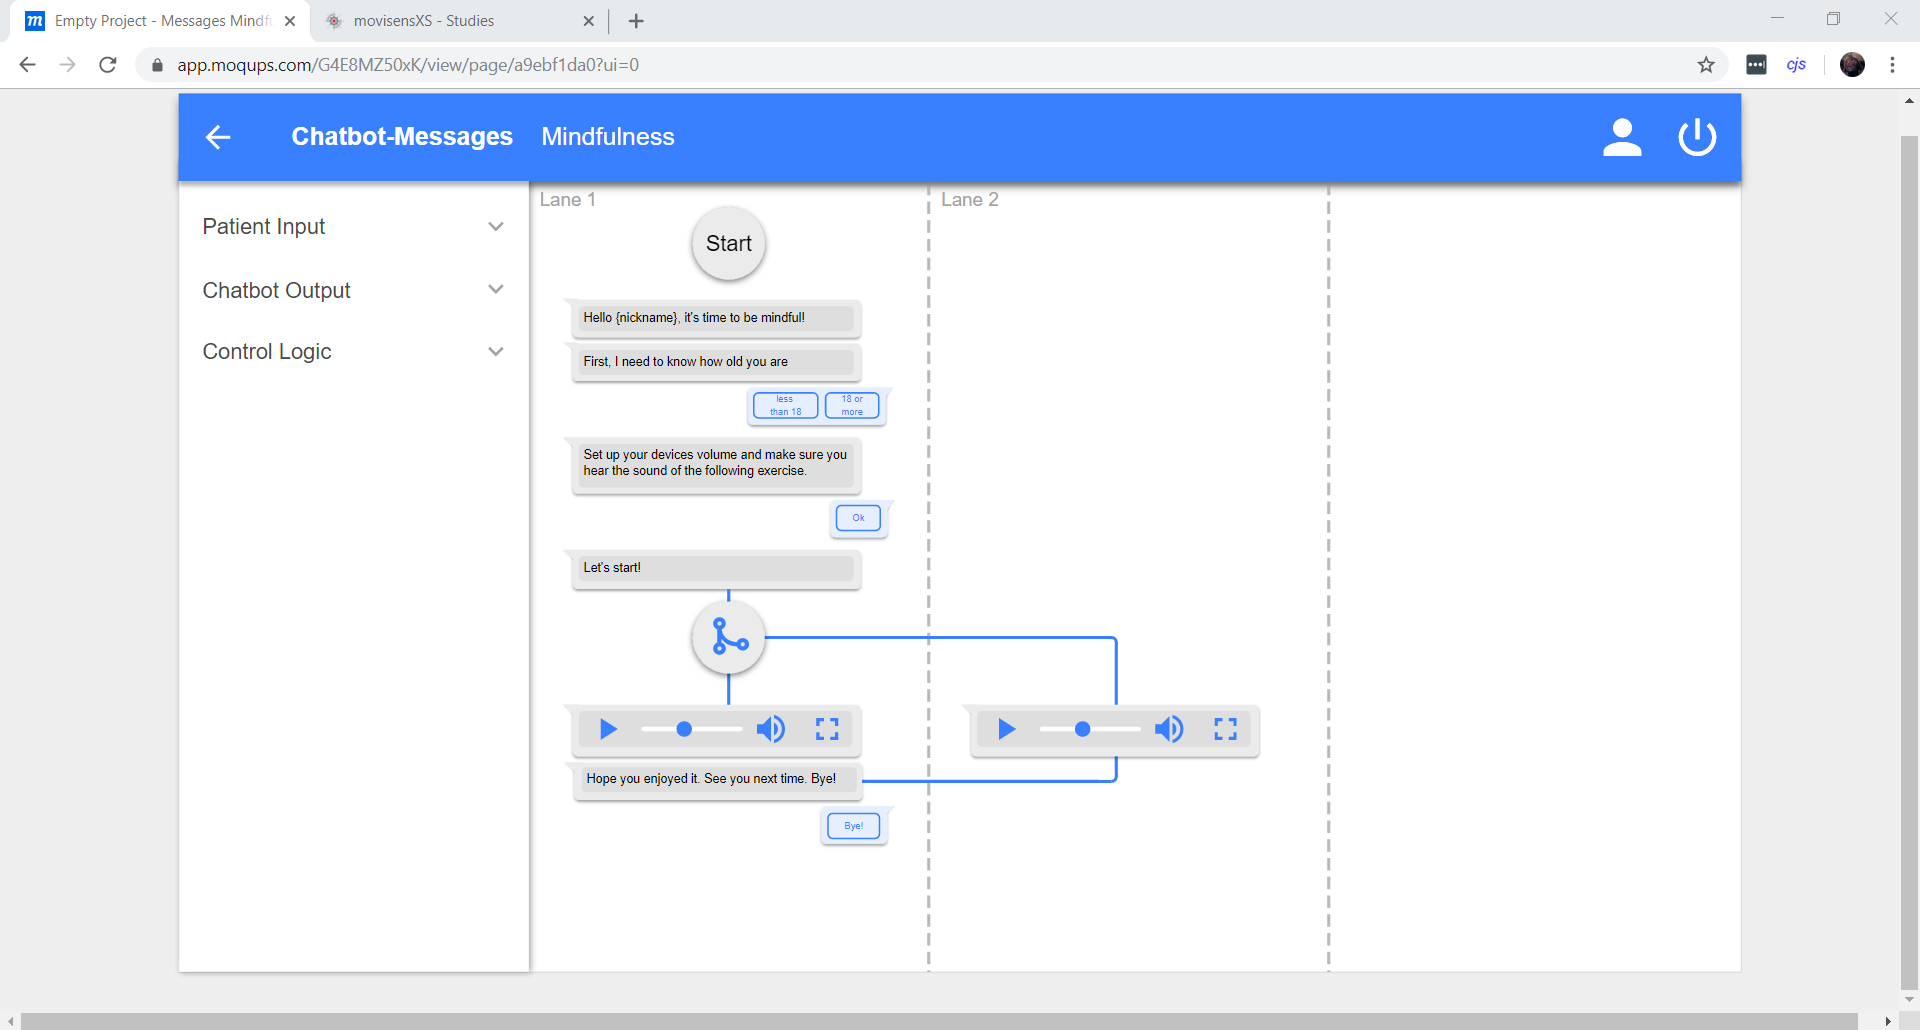
\includegraphics[width=1\textwidth]{pictures/spruenge}
\caption{Architektur des \emph{spruenge}}
\label{spruenge}
\end{figure}

Die Ausgaben des Chatbots werden in einer grauen Sprechblase abgebildet. Die Sprechblase ist nach links orientiert ausgerichtet. Die Eingabeformate des Anwenders werden in einer blauen Sprechblase dargestellt. Diese sind nach rechts orientiert. Der Gesprächsverlauf wird in sogenannten \emph{Lanes} dargestellt. Zunächst wird dieser innerhalb einer \emph{Lane} angelegt. Wird ein alternativer Gesprächsverlauf dargeboten, so wird dies durch eine Condition, in Form eines runden Elements, angedeutet. Dieses runde Element kann entsprechend der Bedingung eingestellt werden und bestimmt, in welcher \emph{Lane} der alternative Gesprächsverlauf weitergeführt wird. 


Hinsichtlich der Darstellung der Konversationen beurteilten die Probanden diese als voll und ganz verständlich. Dies lässt sich auch in den Freitexten der Probanden wiederfinden. Knapp achtundachtzig Prozent der Aussagen äußern sich positiv über die Darstellung der Konversationen. So gefällt im allgemeinen die zeitliche Abfolge, die Gestaltung wie auch die Übersichtlichkeit. 

Die Einstellungsmöglichkeiten der Konversationen empfanden die Probanden im Schnitt als voll und ganz verständlich. Sie tendierten leicht zu zumeist verständlich. Ein Proband äußerte sich auch positiv über die Möglichkeit, die Konversation in dem dargestellten Ablauf zu bearbeiten. Ein weiterer merkte die vielen Einstellungsmöglichkeiten an, die dennoch nicht visuell erschlagen.

Bezüglich des Konversationsverlaufs und dessen Übersichtlichkeit äußerten die Probanden, dass diese im Schnitt als sehr gut empfunden wird. Dabei gibt es eine sehr leichte Tendenz zu \emph{als gut empfunden}. Die Freitext-Aussagen bekräftigen dies. Hier wird vermehrt auf die Übersichtlichkeit eingegangen. Die Hälfte der Probanden-Aussagen gaben dies unter den Punkten an, die ihnen am System am besten gefallen haben. Die Hälfte der Probanden gaben unter diese Punkt allgemein an, dass ihnen die Darstellung der Konversationen gefallen hat.

Antwortoptionen eines Konversationsverlaufs wurden im Allgemeinen als Übersichtlich wahrgenommen. Im Schnitt wurde diese als sehr gut bewertet. Keiner der Probanden ging innerhalb der Freitext-Angaben weiter darauf ein.

Verzweigungen innerhalb eines Konversationsverlaufs wurden ebenfalls im Schnitt als sehr gut verständlich empfunden. Es ließ sich hier eine leichte Tendenz zur Einschätzung \emph{gut verständlich} erkennen. Ein Proband schrieb, dass die Konditionen Sinn ergeben. Eine weitere Anmerkung weißte allerdings auf die Befürchtung hin, dass die Lane-Anordnung, die bei einer Verzweigung entsteht, bei mehr als drei Verzweigungen kompliziert werden könnte. Außerdem konnte ein Proband aus der Grafik nicht genau ableiten, welche Bedingungen und Entscheidungen zusammenhängen. 

Die Werkzeugpalette zur Erstellung des Konversationsverlaufs wurde im Schnitt als sehr Übersichtlich, mit einer Tendenz zu gut Übersichtlich, wahrgenommen. Hier wurde von einem Probanden angemerkt, dass viele Einstellungsmöglichkeiten angeboten werden, ohne mit diesen visuell zu erschlagen. Auch die Aussage, dass die Konditionen Sinn ergeben, bekräftigen das Ergebnis der Fragebogen-Auswertung. 

\subsubsection{Ergebnisbeschreibung der Sichtbarkeitsregeln}

Die Sichtbarkeitsregeln unterscheiden sich maßgeblich von dem Konzept der Sprünge, die zuvor betrachtet wurden. Die Sichtbarkeit eines Elements, welches einen Teil einer Konversation darstellt, wird anhand eines Icons, in Form eines Auges, angedeutet. Die Einstellungsmöglichkeit der Sichtbarkeit erscheint, sobald der Nutzer den Mauszeiger über eines der Elemente bewegt. Anschließend kann, durch ein Klick auf das Auge, die Einstellung der Sichtbarkeitsregel vorgenommen werden. Hier wird entschieden, für welche Gruppe das entsprechende Element im Gesprächsverlauf erscheint. Diese Einstellung wird anhand einer Regel festgelegt. Diese Regel prüft ein oder mehrere Variablen ab. Wurde eine solche Regel einem Element hinterlegt, so erscheint an diesem das Augensymbol dauerhaft, wie in Abbildung \ref{sichtbarkeit} zu sehen ist. Darüber hinaus werden die Dialoge des Konversationsverlaufs anhand von Forms zusammengesetzt. Diese beinhalten entweder nur einen Chatbot-Output oder Chatbot-Output und Input des Nutzers. 

\begin{figure}[h]
\centering
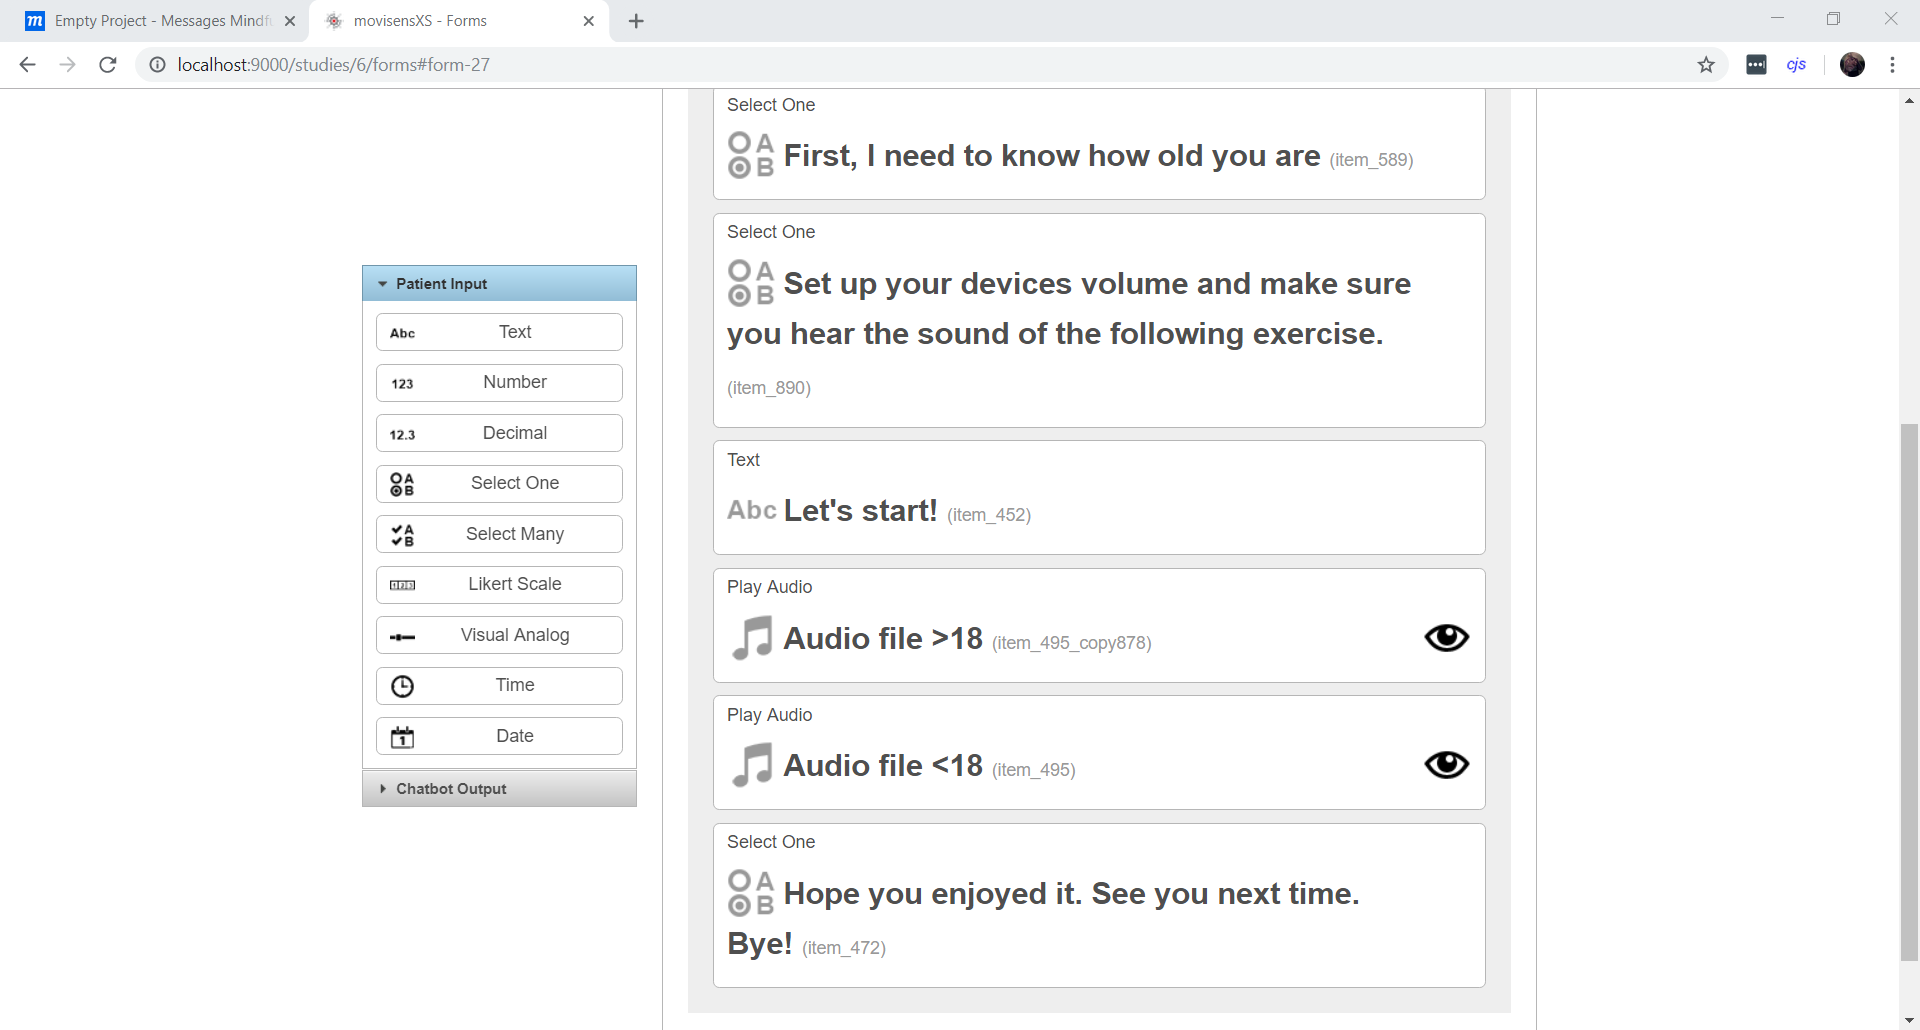
\includegraphics[width=1\textwidth]{pictures/sichtbarkeit}
\caption{Architektur des \emph{sichtbarkeit}}
\label{sichtbarkeit}
\end{figure}

Dieses Konzept wurde ebenfalls von den Probanden bewertet. Aus der Bewertung lassen sich folgende Aussagen treffen. 

Auf Basis der Sichtbarkeitsregel und dem Design des Konversationsverlaufs wurde die Darstellung der Konversationen generell als zumeist verständlich bewertet. Es lässt sich eine leichte Tendenz erkennen, die angibt, dass die Darstellung zum Teil verständlich ist. Die Probandenaussagen der Freitexte untermauern die Bewertung. Es wurden bezüglich der Darstellung keine Punkte genannt, die den Probanden besonders positiv hervorstach. Hingegen wurden mehrere Aussagen getroffen, welche die Darstellung der Konversationen bemängeln. Etwas mehr als sechzig Prozent der Nutzer haben sich diesbezüglich negativ geäußert.

Die Einstellungmsöglichkeiten der Konversationen wurde von den Probanden ebenfalls als zumeist verständlich, mit leichter Tendenz zu zum Teil verständlich, wahrgenommen. Hier wurde in knapp achtunddreißig Prozent der Aussagen die Vielfalt der Einstellungsmöglichkeiten positiv hervorgehoben. Auch die Kategorisierung der Einstellungsmöglichkeiten wurde einmal positiv erwähnt. Hingegen wurde ebenfalls in achtunddreißig Prozent der Aussagen die Unterscheidbarkeit zwischen Chatbot-Output und Patient-Input Elementen, innerhalb des Werkzeugkastens, bemängelt. Diese unterscheiden sich kaum. 

Als gut, mit starker Tendenz zu eher gut, wurde im Schnitt die Übersichtlichkeit des Konversationsverlaufs bewertet. Vier der Freitextaussagen bemängeln die Übersicht der Konversationen. Zum einen sei der zeitliche sowie der generelle Verlauf schwer nachvollziehbar.

Die Übersichtlichkeit der Antwortoptionen innerhalb eines Konversationsverlauf wurden von den Probanden im Schnitt als gut empfunden. Die durchschnittliche Bewertung weist dabei eine starke Tendenz zu \emph{eher gut} auf. Dies lässt sich auch in den schriftlichen Aussagen der Probanden wiederfinden. Vier Aussagen äußern sich negativ zur Darstellung des Verlaufs. Keine Aussage geht speziell auf die Antwortoptionen ein. 

Als eher gut bewerteten die Probanden im Schnitt die Verständlichkeit der Verzweigungen innerhalb einer Konversation. Hierzu passen die Freitext-Aussagen der Probanden, die angaben, dass die Übersicht des zeitlichen Verlaufs fehle und somit für diese Probanden eher schwer nachvollziehbar ist. Diese Aussage trafen fünfzig Prozent. Ein Proband wies außerdem darauf hin, dass ihm unklar ist, woher die Variable stammt, die für die Verzweigung überprüft wird. 

Im Schnitt bewerteten die Probanden die Übersichtlichkeit der Werkzeugpalette zur Erstellung des Konversationsverlaufs als gut. Auch hier zeigte sich eine starke Tendenz zur schlechteren Bewertung. Hier merkte ein Probanden an, dass der Zustand der Werkzeugpalette beim Öffnen des Konversationsreiters, hinderlich ist. Die Einstellungsmöglichkeiten des Chatbot-Outputs sind durch diesen leicht zu übersehen. 

\section{Ergebnisbeschreibung der Abschlussfragerunde}

Zur Gesamtbewertung der Systeme wurden die Probanden abschließend zur Studie über die Eigenschaften der Systeme befragt. Die Probanden sollten erläutern was sie innerhalb der verschiedenen Konzepte als hilfreich und nicht hilfreich empfunden haben. Außerdem sollten sie darauf eingehen, welche Punkte sie in den Ansätzen vermisst haben und was ihnen besonders gut gefallen hat. Befragt wurden sie direkt zum Konfigurations- und Konstruktionsprinzip sowie den Ansätzen der Steuerung des Konversationsflusses durch Sichtbarkeitsregeln und Sprünge. Nachfolgend werden die Ergebnisse dargestellt.

\subsection{Ergebnissbeschreibung Konfigurationsprinzip}

Insgesamt nannten die Probanden siebenundfünfzig Punkte zum Konfigurationsprinzip. Etwas mehr als die Hälfte der Punkte betreffen die Frage, was die Probanden als besonders hilfreich empfanden. Siebzehn Prozent der Aussagen wurden von den Probanden auf die Nachfrage, was ihnen weniger oder nicht hilfreich erschien, getätigt. Auf die Frage, was ihnen gut gefallen habe, gaben die Probanden zehn Punkte an. Dies macht ebenfalls siebzehn Prozent der Aussagen aus. Die restlichen fünfzehn Prozent der angesprochenen Punkte bezogen sich auf die Bitte zu erläutern, was sie an der Umsetzung vermisst haben. 

\paragraph{Hilfreich}Die Hälfte der Probanden empfanden besonders die zeitliche Darstellung als hilfreich. Ein Proband beschrieb, dass das Zusammenbringen der Einstellungen und des zeitlichen Ablaufs der Übersicht beiträgt. Ein weiterer ging darauf ein, dass der Zeitstrahl gut interpretierbar ist. Auch da dieser konsistent nach rechts fortlaufend ist. Knapp achtunddreißig Prozent der Probanden äußerten auch, dass die Darstellung generell als übersichtlich empfunden wurde. Weitere Aussagen bekräftigen diese Äußerung. So wurde das System generell als benutzerfreundlich eingestuft. Unter anderem wurde dies durch die Anlehnung an das bekannte Material Design von Google begründet. Auch wurde angemerkt, dass wichtige Informationen und Funktionen im Vordergrund stehen und auch auf die Funktionen reduziert wurde, die für einen entsprechenden Chatbot benötigt werden. Des weiteren wurden die zeitlichen Abhängigkeiten als gut einsehbar empfunden. Hierzu gab es zwei Aussagen die dies hervorhoben. Zwei Anmerkungen bezogen sich auf die farbliche Kodierung der Trigger-Arten. Die Unterscheidung dieser innerhalb der zeitlichen Darstellung wurde positiv empfunden. Auch die Auflistung der Konversationen innerhalb der Darstellung wurde positiv angemerkt. Die Suchfunktion erleichtere das Finden einzelner Konversationen. Dies äußerten ebenfalls zwei Probanden.


\paragraph{Nicht hilfreich}Zwei Probanden konnten keine Aussage darüber treffen, was sie als nicht hilfreich empfanden. Vier weitere Probanden hingegen gaben an, dass die Legende, die in der Darstellung der Umsetzung vorfanden, eher irritierend wahrnahmen. Hier fehlte ihnen eine ausführliche Erklärung der farblichen Kodierung. Außerdem wurden die Icons, die in der zeitlichen Übersicht auftauchten,in der Legende vermisst. Ein weiterer Proband wünschte sich die Möglichkeit, die Konversationen innerhalb der zeitlichen Darstellung klickbar zu gestalten, um daraufhin beispielsweise die Trigger-Einstellungen der entsprechenden Konversation zu öffnen. Des weiteren irritierte einen Probanden die Aufteilung zwischen den Abhängigen Konversationen.

\paragraph{Gut Gefallen} Auf die Frage, was den Probanden an der Umsetzung besonders gut gefallen habe, konnte ein Proband keine Aussage treffen. Siebenunddreißig Prozent der Probanden hingegen gaben an, dass ihnen die zeitliche Darstellung der Konversationen besonders gut gefiel. Ein Proband merkte dabei an, dass auf diese Weise die Belastung der Therapie-Teilnehmer auf einen Blick  einsehbar ist. Auch wurden von weiteren siebenunddreißig Prozent angegeben, dass die Konversation und Trigger gut ineinander greifen. Gefühlt müssen weniger Einstellungsschritte vorgenommen werden und der Fluss dieser wirkt klarer und konsistenter.

\paragraph{Gefehlt} Drei Probanden konnten keine Aussage darüber treffen, was sie an dieser Form der Umsetzung vermisst haben. Fünfundfünzig Prozent der genannten Punkte gingen auf fehlende Hilfestellungen ein. Zum einen wünschen sich die Probanden Anleitungen beziehungsweise Tutorials zur Einführung. Zum anderen vermissten sie Tooltips, die Informationen zu verschiedenen Funktionen und Elementen offenlegen. Desweiteren wünschen sie sich eine Funktion hinter den einzelnen Elementen innerhalb der Zeitdarstellung. Zwei Probanden beschrieben, dass ihnen eine hinterlegte Funktion fehlt, die durch das Anklicken eines solchen Elements ausgelöst wird. Gewünscht wurde hier das Öffnen der Einstellungsmöglichkeiten oder Anzeigen von zugehörigen Informationen der Trigger-Einstellungen. Zusätzlich wünschten sich zwei weitere Probanden eine ausführlichere Legende die mehr Informationen über die Farben und Symbole bietet.


\subsection{Ergebnissbeschreibung Konstruktionsprinzip}

Die Abschlussfragerunde ergab sechzig Aussagen. Achtzehn Prozent der Aussagen bezogen sich auf die Frage, welche Eigenschaften dieser Form der Umsetzung, als besonders Hilfreich erfahren wurden. Auf die Frage hin, welche Eigenschaften als hinderlich empfunden wurden, konnten fünfunddreißig Punkte genannt werden. Diese machen fünfunddreißig Prozent der Abschlussfragerunde aus. Hingegen bezogen sich achtundzwanzig Prozent der Aussagen auf die Frage was den Probanden an dieser Form der Umsetzung besonders gut gefallen hat. Elf Punkte wurden von den Probanden genannt, die sie am System vermisst haben. Dies macht ebenfalls achtzehn Prozent der Aussagen über die Umsetzung aus. 

\paragraph{Hilfreich}Zwei Probanden konnten keine Antwort auf die Frage geben, was sie an dieser Umsetzungsform besonders hilfreich empfanden. Sechsunddreißig Prozent der Antworten gaben an, dass sie insbesondere die farbliche Kodierung der Bausteine als besonders hilfreich empfanden. Somit konnten Beziehungen zwischen Bausteinen besser nachvollzogen werden. Eine weitere Anmerkung eines Probanden unterstützt diese Erklärung. So sagte dieser aus, dass die Farben dabei halfen, sich im Baum zu orientieren. Rote Elemente befinden sich oben, gelbe in der Mitte und Grüne befinden sich in der Darstellung unten. Dies unterstützt bei der Orientierung. Siebenundzwanzig Prozent der Probanden äußerten, dass die grafische Darstellung hilfreich war. So hatten diese mehr Infos auf einem Blick und konnte die Abhängigkeiten gut einsehen. Achtzehn Prozent der Probanden gingen auf die Navigation innerhalb des Prototyps ein. So empfanden sie die Navigation zur Baum-Darstellung als hilfreich. Diese war klar und half dabei sich schneller zurecht zu finden und den Baum mit den entsprechenden Trigger-Einstellungen aufzurufen. Ein weiterer Proband ging auf die vielen Anordnungsmöglichkeiten der Bausteine ein. 


\paragraph{Nicht hilfreich}Die Mehrheit der Aussagen aller Probanden, bezieht sich auf die Übersichtlichkeit der Umsetzungsform, sowie fehlende Erklärungen. So bezogen sich neunundzwanzig Prozent der Antworten auf die fehlende Übersicht. Angemerkt wurde hier die fehlende Möglichkeit die Darstellung des Baums zu vergrößern und zu verkleinern. Außerdem empfanden die Probanden die Darstellung als zu komplex und schlecht überschaubar, sobald die Anzahl der Verbundenen Bausteine etwas wächst. Weitere vierundzwanzig Prozent der Aussagen betrafen die fehlenden Erklärungen. So vermissten die Probanden Toolboxen und Anleitungen um sich bei dieser Darstellung besser zurecht zu finden. Vierzehn Prozent der angesprochenen Punkte äußerten sich über den Workload der Darstellungsform. So äußerten Probanden, dass für diese eine längere Auseinandersetzung notwendig ist, um die Darstellungsform zu verstehen und zu bedienen. Dies liege unter anderem auch daran, dass die Konversationen und der zeitliche Ablauf unverbunden wirken. Ein Proband antwortete, dass die Vielzahl an Navigationsmöglichkeiten nicht zur Übersicht beitragen. Ein weiterer ging auf die Suche eines Moduls, beziehungsweise einer Konversation, innerhalb des Baums ein. Dieser fand es störend, dass die Suche nach einem Modul aus durchsuchen des Baums besteht. Ebenfalls äußerte ein Proband, dass die Platzierungsart der einzelnen Blöcke als hinderlich empfunden wurde.

\paragraph{Gut Gefallen}Besonders gut gefallen hat den Probanden die Farbliche Trennung der Bausteine.  Fünfunddreißig Prozent der Aussagen äußerten sich hierzu positiv. Auch die Drag and Drop-Funktion hoben die Probanden positiv hervor. Auf diese beziehen sich neunundzwanzig Prozent der genannten Punkte. Knapp zwölf Prozent gefällt das Zusammenbauen des Baums, unter anderem durch dessen Flexibilität in der Anordnung und Gestaltung. Weitere Punkte die gut gefallen, sind die grafische Darstellung, die gute Nachvollziehbarkeit der Einstellungsmöglichkeiten, die Intuitive Navigation durch die Reiter, sowie die vorhandenen Informationen innerhalb des Baums. Diese Aussagen nehmen einen Anteil von knapp sechs Prozent aller genannten Punkte ein.

\paragraph{Gefehlt}Vermisst haben die Probanden folgende Funktionen: eine Suchfunktion nach Modulen, Erklärungen zur Bedienung und Bedeutung beispielsweise der Farben, sowie einen besseren Überblick über den Studienablauf. Jeweils siebenundzwanzig Prozent der Aussagen bezogen sich auf diese Punkte. Neben diesen wurde von einem Probanden der Sinn des Dashboards angesprochen. Dessen Funktion ging für den Probanden nicht genau hervor. Ein weiterer Punkt spricht an, dass die Arbeitsbelastung des Nutzers nicht aus dem Baum hervorgeht.

\subsection{Ergebnissbeschreibung Sprünge}

\paragraph{Hilfreich}

\paragraph{Nicht hilfreich}

\paragraph{Gut Gefallen}

\paragraph{Gefehlt}

\subsection{Ergebnissbeschreibung Sichtbarkeitsregeln}

\paragraph{Hilfreich}

\paragraph{Nicht hilfreich}

\paragraph{Gut Gefallen}

\paragraph{Gefehlt}

%%%%%%%%%%%%%%%%%%%%%%%%%%%%%%%%%%%%%%%%%%%%%%%%%%%%%%%%%%%%%%%%%%%%%%%%%%%%%%%%%%%%%%%%%%%%%%%%%%%%%%


\begin{figure}[h]
\centering
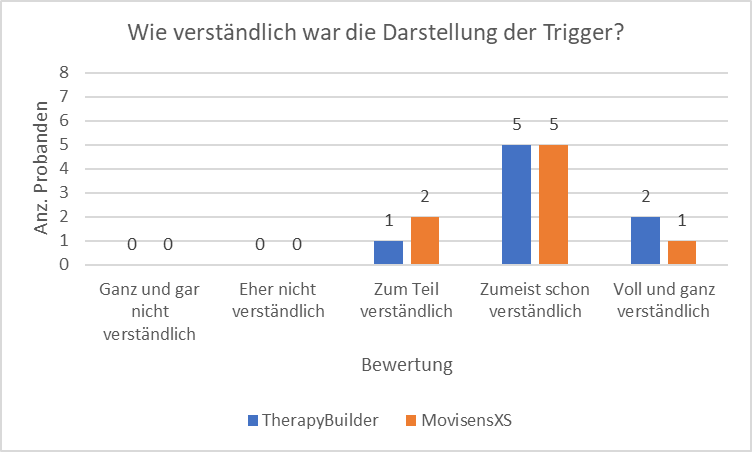
\includegraphics[width=1\textwidth]{pictures/diagramme/triggerdarstellung}
\caption{Architektur des \emph{konfiguration}}
\label{triggerdarstellung}
\end{figure}

\begin{figure}[h]
\centering
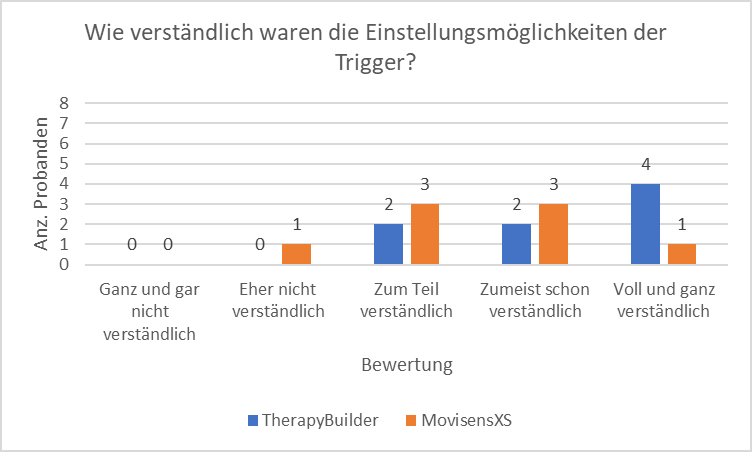
\includegraphics[width=1\textwidth]{pictures/diagramme/triggereinstellung}
\caption{Architektur des \emph{konfiguration}}
\label{triggereinstellung}
\end{figure}

\begin{figure}[h]
\centering
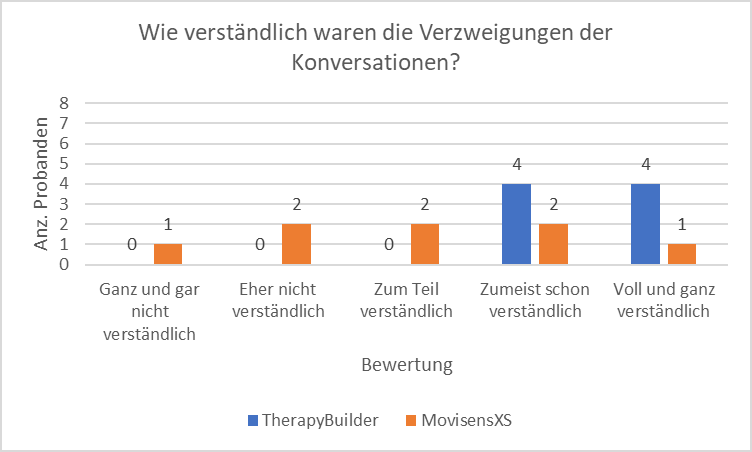
\includegraphics[width=1\textwidth]{pictures/diagramme/konversationverzweigung}
\caption{Architektur des \emph{konfiguration}}
\label{konversationverzweigung}
\end{figure}

\begin{figure}[h]
\centering
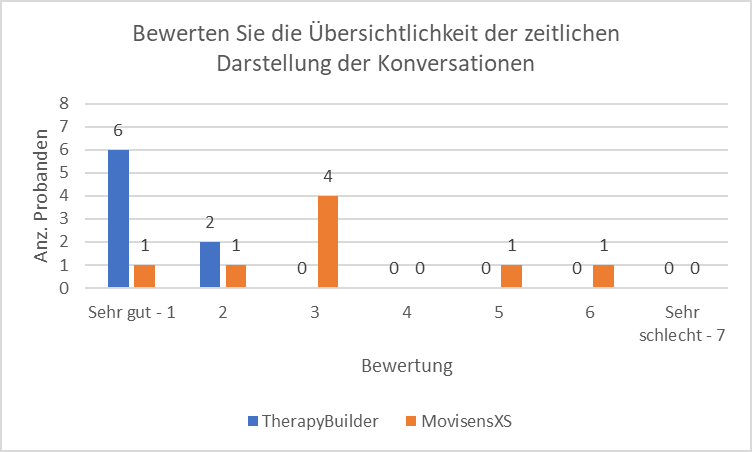
\includegraphics[width=1\textwidth]{pictures/diagramme/konversationzeitldarstellung}
\caption{Architektur des \emph{konfiguration}}
\label{konversationzeitldarstellung}
\end{figure}

\begin{figure}[h]
\centering
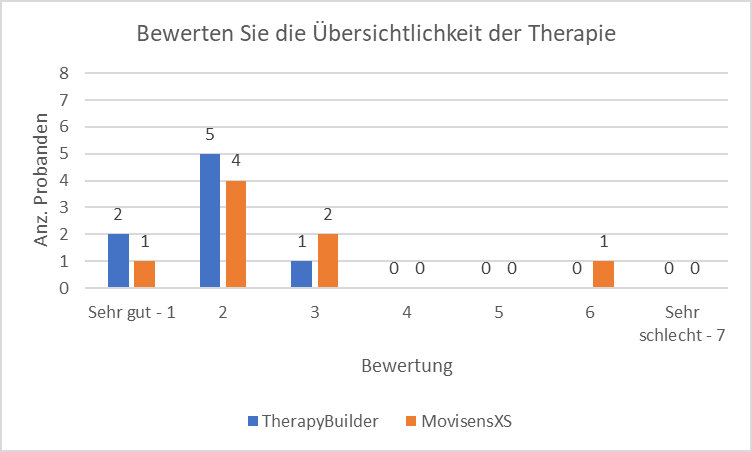
\includegraphics[width=1\textwidth]{pictures/diagramme/therapieuebersicht}
\caption{Architektur des \emph{konfiguration}}
\label{therapieuebersicht}
\end{figure}


\begin{figure}[h]
\centering
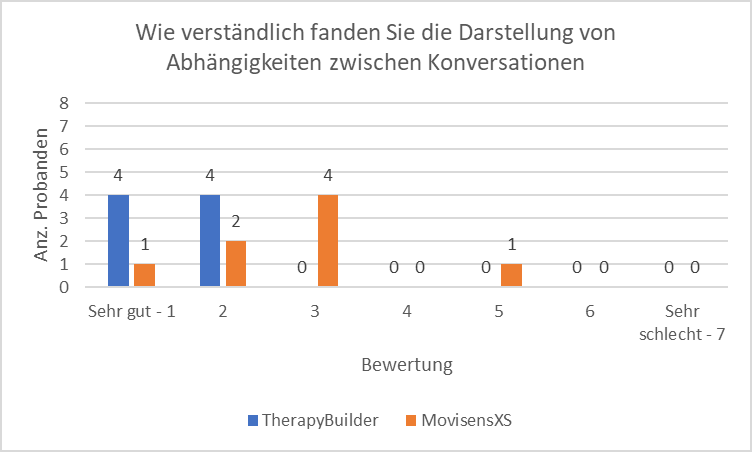
\includegraphics[width=1\textwidth]{pictures/diagramme/konversationenabhaeng}
\caption{Architektur des \emph{konfiguration}}
\label{konversationenabhaeng}
\end{figure}

\begin{figure}[h]
\centering
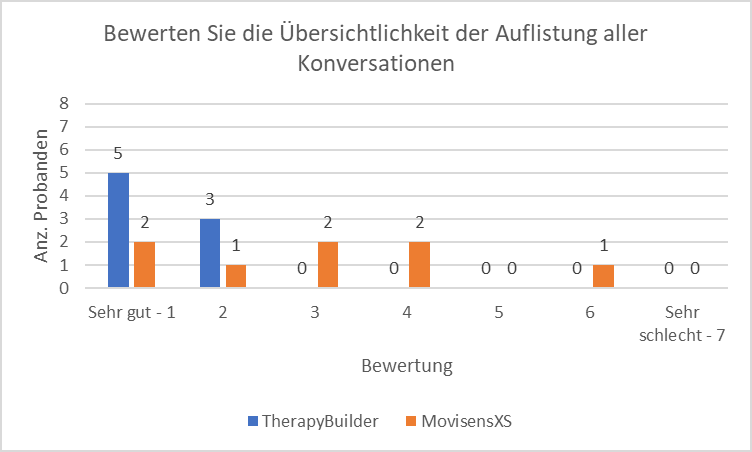
\includegraphics[width=1\textwidth]{pictures/diagramme/konversationenuebersicht}
\caption{Architektur des \emph{konfiguration}}
\label{konversationenuebersicht}
\end{figure}

\begin{figure}[h]
\centering
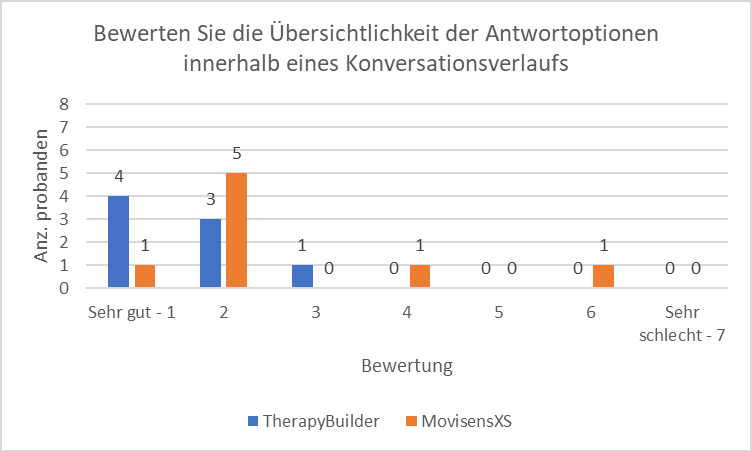
\includegraphics[width=1\textwidth]{pictures/diagramme/antwortoptkonv}
\caption{Architektur des \emph{sichtbarkeit}}
\label{antwortoptkonv}
\end{figure}

\begin{figure}[h]
\centering
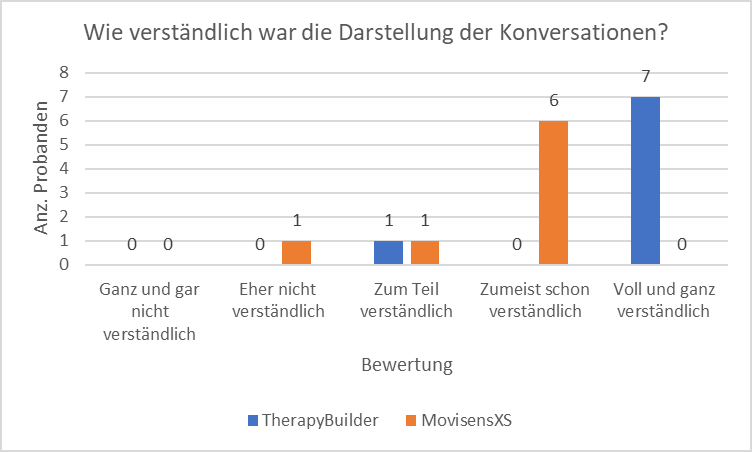
\includegraphics[width=1\textwidth]{pictures/diagramme/konversationdarstellung}
\caption{Architektur des \emph{konfiguration}}
\label{konversationdarstellung}
\end{figure}

\begin{figure}[h]
\centering
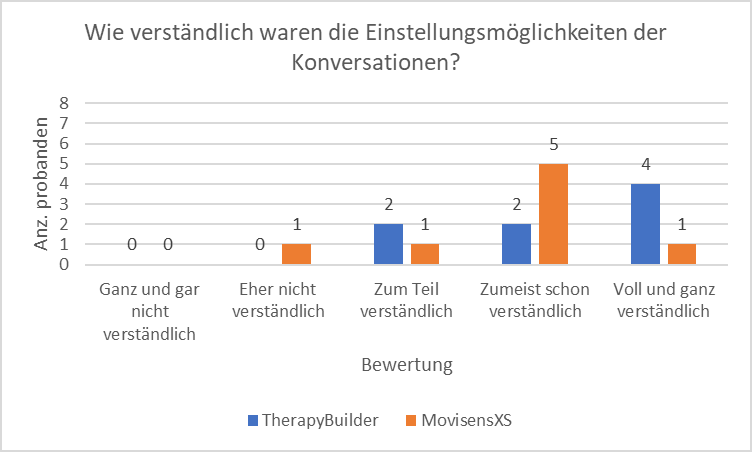
\includegraphics[width=1\textwidth]{pictures/diagramme/konversationeinstellung}
\caption{Architektur des \emph{konfiguration}}
\label{konversationeinstellung}
\end{figure}



\begin{figure}[h]
\centering
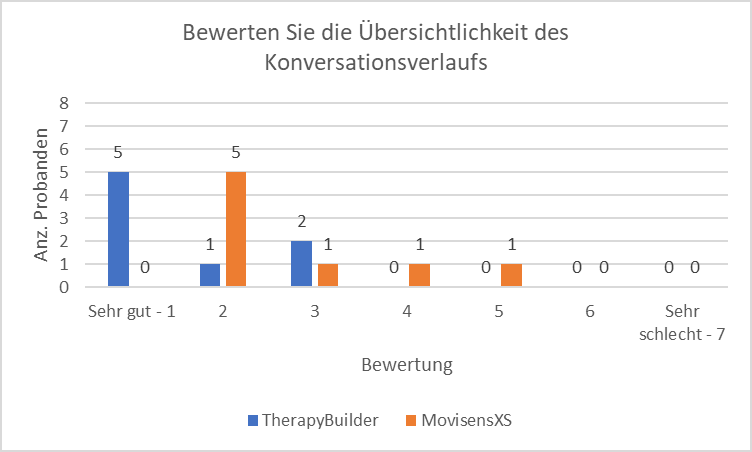
\includegraphics[width=1\textwidth]{pictures/diagramme/konversationverlfueber}
\caption{Architektur des \emph{konfiguration}}
\label{konversationverlfueber}
\end{figure}

\begin{figure}[h]
\centering
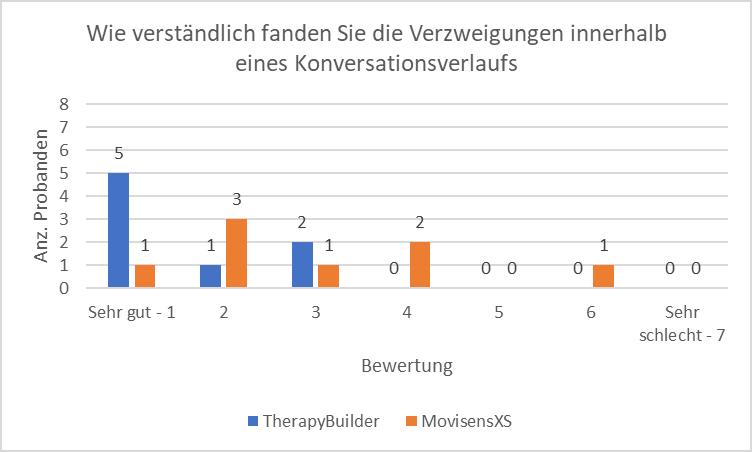
\includegraphics[width=1\textwidth]{pictures/diagramme/konvverzweig}
\caption{Architektur des \emph{konfiguration}}
\label{konvverzweig}
\end{figure}


\begin{figure}[h]
\centering
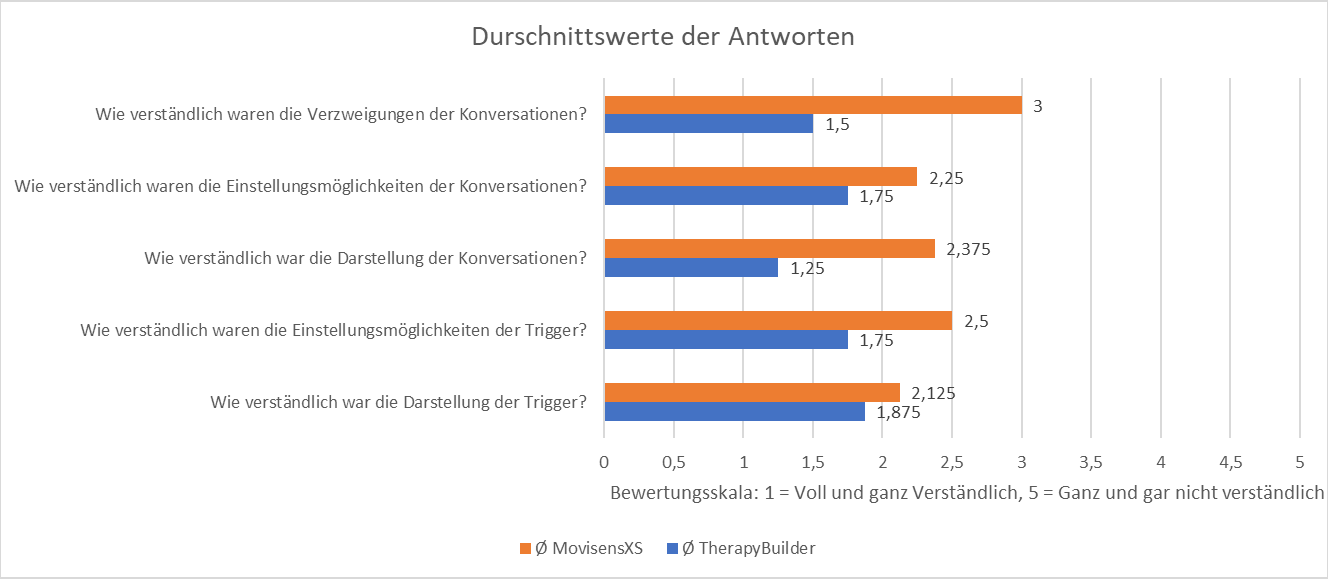
\includegraphics[width=1\textwidth]{pictures/diagramme/antwortendurchsch1}
\caption{Architektur des \emph{konfiguration}}
\label{antwortendurchsch1}
\end{figure}

\begin{figure}[h]
\centering
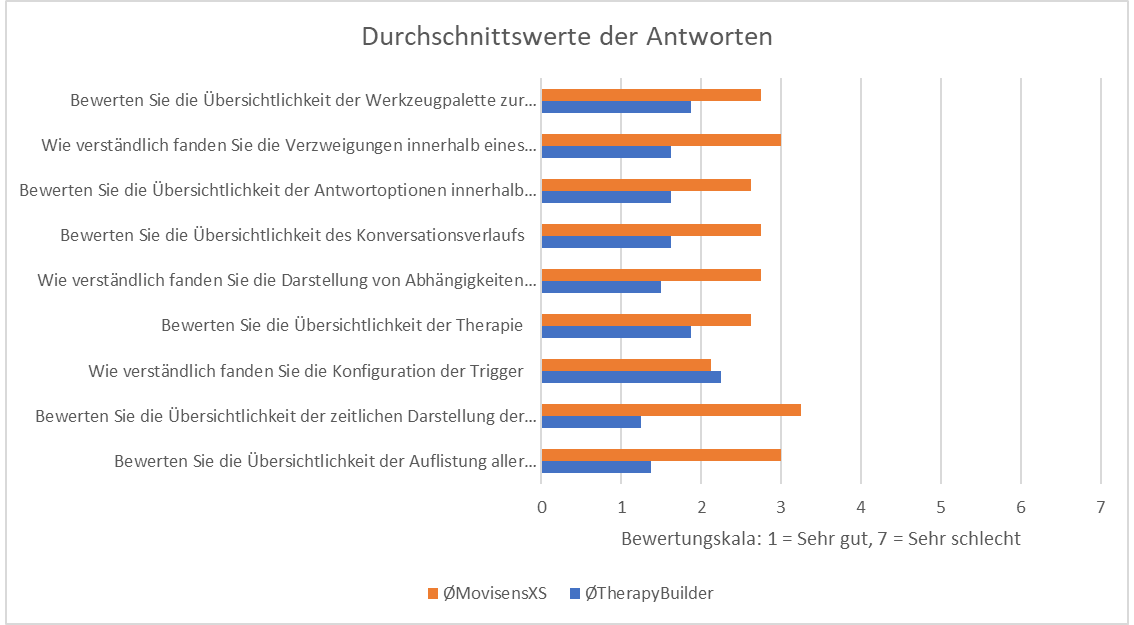
\includegraphics[width=1\textwidth]{pictures/diagramme/antwortendurchsch2}
\caption{Architektur des \emph{konfiguration}}
\label{antwortendurchsch2}
\end{figure}



